\documentclass{ctexbeamer}
\usetheme{Madrid}
\setmainfont{Times New Roman}
\setCJKsansfont{宋体}

% workaround https://github.com/josephwright/beamer/issues/337
\makeatletter
\def\beamer@framenotesbegin{% at beginning of slide
  \usebeamercolor[fg]{normal text}
  \gdef\beamer@noteitems{}%
  \gdef\beamer@notes{}%
}
\makeatother

\usepackage{pgfpages}
\setbeameroption{show notes on second screen}

\title[数据库的自然语言接口]{数据库的自然语言接口关键技术研究}
\author{胡玮文}
\institute[SCUT]{华南理工大学}
\date{2020/6/2}
\logo{\includegraphics[height=1.5cm]{figure/SCUT_logo.png}}

\AtBeginSection[]
{
  \begin{frame}
    \frametitle{目录}
    \tableofcontents[currentsection]
  \end{frame}
}

\begin{document}
\frame{\titlepage}
\note{
  \begin{itemize}
    \item 大家好
    \item 自我介绍
    \item 题目
  \end{itemize}
  Time: 00:18
}
\logo{}

\def\sql#1{\texttt{#1}}
\def\kw#1{\textcolor{blue}{#1}}
\def\SELECT{\kw{SELECT }}
\def\FROM{\kw{FROM }}
\def\JOIN{\kw{JOIN }}
\def\WHERE{\kw{WHERE }}
\def\AS{\kw{AS }}
\def\ON{\kw{ON }}
\def\AND{\kw{AND }}
\def\GROUPBY{\kw{GROUP~BY }}
\def\ORDERBY{\kw{ORDER~BY }}
\def\LIMIT{\kw{LIMIT }}
\def\DESC{\kw{DESC }}
\def\DISTINCT{\kw{DISTINCT }}

\newlength{\sqlindentwidth}
\settowidth{\sqlindentwidth}{\sql{aaaa}}
\def\SQLINDENT{\-\hspace{\sqlindentwidth}}


\begin{frame}
  \frametitle{目录}
  \tableofcontents

  \note{Time: 00:25}
\end{frame}

\section{背景}
\begin{frame}
  \frametitle{数据库的自然语言接口}
  日常生活中,人们每天都在和无数数据库打交道
  \note{
    \begin{itemize}
      \item 生活中很多信息系统,数据库
      \item 普通用户很少与数据库直接交互,需要专业,SQL,但普通用户不具有这样的专业能力
    \end{itemize}
  }
  \begin{figure}[]
    \includegraphics[page=12]{figure/figures.pdf}
    \caption{当前与数据库交互的方式}
  \end{figure}
  \note{
    普通用户通过用户界面与数据库交互

    Time: 01:00
  }
\end{frame}
\begin{frame}
  \frametitle{数据库的自然语言接口}
  \begin{figure}
    \includegraphics[page=11]{figure/figures.pdf}
    \caption{通过自然语言接口与数据库直接交互}
  \end{figure}
  \begin{block}{意义}
    广大用户首次获得了直接面对大数据的能力
    \note{
      大数据时代,数据产生快,分析数据水平不够。帮助用户获取分析任何信息,探索。\par
    }
  \end{block}
  \note{
    如何实现?(过渡)

    Time: 01:25
  }
\end{frame}

\begin{frame}
  \frametitle{自然语言到SQL转换任务}
  实现数据库的自然语言接口的方式之一:将自然语言转换为SQL
  \note{方法之一。所有现有数据库都能获得自然语言接口的能力。\par}
  \begin{figure}
    \includegraphics[page=13]{figure/figures.pdf}
    \caption{通过自然语言到SQL转换与数据库交互}
  \end{figure}
  \note{目标:构建一个这样的转换器\par}
  \note{
    过渡:为了实现这个目标,之前也有不少努力。

    Time: 01:45
  }
\end{frame}
\begin{frame}
  \frametitle{SParC数据集}
  SParC数据集是跨领域的,上下文相关的自然语言到SQL转换任务数据集
  \note{
    \begin{itemize}
      \item 内容包括数据库架构,以及多轮与数据库的交互
      \item 每轮交互包括一个自然语言的查询和对应的SQL语句
      \item 目标:构建转换器,输入:数据库架构,自然语言查询。输出:对应SQL语句
      \item 介绍跨领域
      \item 介绍上下文相关
    \end{itemize}
  }
  \begin{columns}
    \column{0.6\textwidth}
    What are all the airlines?

    \sql{\SELECT * \FROM AIRLINES}

    \vspace{0.2cm}
    Of these, which is Jetblue Airways?

    \sql{\SELECT * \FROM AIRLINES \WHERE Airline = "JetBlue Airways"}

    \vspace{0.2cm}
    What is the country corresponding it?

    \sql{\SELECT Country \FROM AIRLINES \WHERE Airline = "JetBlue Airways"}

    \column{0.35\textwidth}
    \begin{figure}
      \includegraphics[width=\textwidth,trim=30 10 10 10,clip]{figure/schema_flight_2.pdf}
      \caption{数据库架构}
    \end{figure}
  \end{columns}
\end{frame}

\section{提出的方法}
\begin{frame}
  \frametitle{整体架构}
  \begin{figure}
    \includegraphics[page=6,width=\linewidth]{figure/figures.pdf}
    \caption{模型整体架构}
  \end{figure}
  \note{主要:编码器、解码器\par}
  \note{过渡:后面主要介绍本研究中的改进内容}
\end{frame}

\subsection{SQL预处理和后处理}
\begin{frame}
  \frametitle{SQL预处理和后处理}
  \begin{itemize}
    \item SQL中包含冗余的,抽象层次低的结构,将显著影响模型预测的准确率
    \item EditSQL的方案为去除SQL中最为冗余的FROM子句,但并非所有FROM的内容都是冗余的。17.3\%的SQL无法还原
  \end{itemize}
  \begin{example}[去掉FROM子句后将丢失信息]
    Which students have pets?

    \vspace{0.2cm}
    \sql{\SELECT \DISTINCT T1.fname \\
      \SQLINDENT\FROM student \AS T1 \\
      \SQLINDENT\JOIN has\_pet \AS T2 \ON T1.stuid = T2.stuid}

    转换为

    \sql{\SELECT \DISTINCT student.fname}
  \end{example}
\end{frame}
\begin{frame}
  \frametitle{SQL预处理和后处理}
  \framesubtitle{本文方案}
  更细粒度地处理FROM子句,保留必要的信息。仅2.3\%的SQL无法还原

  预处理过程
  \begin{enumerate}
    \item 解析列引用,将引用表达式替换为“表名.列名”的规范形式
    \item 去除所有JOIN子句中的ON部分
    \item 去除FROM子句中用于多对多关联的JOIN子句
    \item 在FROM子句中,去除所有在SQL的其他部分引用过的表。若所有表都被去除,则去除整个FROM子句。
  \end{enumerate}
  后处理过程
  \begin{enumerate}
    \item 将所有在SQL中引用过的表添加到FROM子句中。
    \item 根据外键关系,将数据库中的所有表构造成无向图,并使用Kruskal算法求解包含当前FROM子句中的表的最小生成树,根据生成树的边和节点来重建JOIN子句中的ON部分。
    \item 有多张表时,恢复别名
  \end{enumerate}
\end{frame}
\begin{frame}
  \frametitle{SQL预处理和后处理}
  \framesubtitle{本文方案}
  \begin{example}
    \sql{\SELECT T3.Party\_Theme, T2.Name \FROM party\_host \AS T1 \newline
    \SQLINDENT\JOIN host \AS T2 \ON T1.Host\_ID = T2.Host\_ID \newline
    \SQLINDENT\JOIN party \AS T3 \ON T1.Party\_ID = T3.Party\_ID}


    转换为

    \sql{\SELECT party.Party\_Theme, host.Name}

  \end{example}
  \begin{itemize}
    \item 解析别名\texttt{T2},\texttt{T3}为真正的表名
    \item \texttt{party\_host}是多对多关联表,\texttt{host}和\texttt{party}表均在SELECT子句中被引用过,所以整个FROM子句全部被去除。
  \end{itemize}
\end{frame}

\subsection{上下文编码机制}
\begin{frame}
  \frametitle{上下文编码机制}
  EditSQL使用会话级别RNN编码上下文信息
  \begin{figure}
    \includegraphics[page=8,width=0.9\textwidth]{figure/figures.pdf}
    \caption{EditSQL编码上下文方案}
  \end{figure}
\end{frame}
\begin{frame}
  \frametitle{上下文编码机制}
  BERT等模型经过大规模无标注文本数据预训练,能更好地理解自然语言的上下文信息,如指代、省略等现象。
  \begin{figure}
    \includegraphics[page=9,width=0.9\textwidth]{figure/figures.pdf}
    \caption{本文上下文编码机制}
  \end{figure}
\end{frame}

\subsection{关系编码机制}
\begin{frame}
  \frametitle{关系编码机制}
  \begin{itemize}
    \item 数据库架构中包含有主键,外键等信息。这些信息被以往的很多方法忽略
    \item 本文将数据库架构的编码结合进预训练注意力机制中
      \note{编码有向图}
  \end{itemize}

  \begin{figure}
    \includegraphics[page=10,width=\textwidth]{figure/figures.pdf}
    \caption{关系编码机制示意\footnote{为了展示简洁,标点符号对应的表示已省略,它们全部使用“其他”关系。此处仅展示了部分关系类型。}}
  \end{figure}
\end{frame}

\section{实验}
\begin{frame}
  \frametitle{总体结果}
  \begin{table}
    \begin{tabular}{l|rr}
\hline\hline
                    & 问题准确率 & 交互准确率 \\ \hline
SyntaxSQL-con       & 18.5      & 4.3   \\
CD-Seq2Seq          & 21.9      & 8.1   \\
EditSQL with BERT   & 47.2      & 29.5  \\
本文模型 with BERT   & 54.3      & 34.6  \\
本文模型 with XLNet  & \textbf{58.5} & \textbf{39.6} \\ \hline
\multicolumn{3}{l}{使用标注的历史SQL查询}    \\ \hline
EditSQL with BERT   & 53.4      & 29.2  \\
本文模型 with BERT   & 60.7      & 34.6  \\
本文模型 with XLNet  & \textbf{64.3} & \textbf{39.3}  \\ \hline\hline
\end{tabular}

    \caption{SParC实验总体结果}
  \end{table}
\end{frame}
\begin{frame}
  \frametitle{消融实验}
  \begin{columns}
    \column{0.4\textwidth}
    \begin{itemize}
      \item “无FROM”为EditSQL所用方案
      \item “FROM未引用表”为本文最终采用方案
    \end{itemize}
    \column{0.6\textwidth}
    \framesubtitle{SQL预处理和后处理}
    \begin{figure}
      \includegraphics[height=0.68\textheight]{figure/preprocess.pdf}
      \caption{各种预处理方案对比}
    \end{figure}
  \end{columns}
  \note{
    EditSQL的方案虽然会导致信息丢失,但依然是有助提升性能的。

    要预测的冗余的信息越多,准确率越低
  }
\end{frame}
\begin{frame}
  \frametitle{消融实验}
  \framesubtitle{上下文编码 \& 关系编码机制}
  \begin{table}
    \begin{tabular}{l|rr}
\hline\hline
            & 问题准确率 & 交互准确率 \\ \hline
本文模型     & 58.5      & 39.6  \\
- 上下文编码 & 54.2      & 33.9  \\
- 关系编码   & 57.1      & 38.9  \\ \hline\hline
\end{tabular}

    \caption{消融实验结果}
  \end{table}
  \begin{block}{实验对比结果}
    \begin{itemize}
      \item 上下文编码机制虽然简单,但效果显著
      \item 关系编码机制带来较小提升
    \end{itemize}
  \end{block}
  \note{
    关系编码提升小,可能原因:
    \begin{itemize}
      \item 预训练模型能从内容中较好理解关系,编码仅是锦上添花
      \item 编码未能良好融入预训练模型后
    \end{itemize}
  }
\end{frame}
\begin{frame}
  \frametitle{错误分析}
  \begin{columns}
    \column{0.4\textwidth}
    \begin{itemize}
      \item 大多数错误出现在单个子查询内
        \note{大多查询不包括子查询和组合结构。其预测准确率也很低}
      \item 较高层次的查询骨架错误和较低层次的列选择错误都较多
      \item 语法错误几乎没有
    \end{itemize}
    \column{0.6\textwidth}
    \begin{figure}
      \includegraphics[height=0.7\textheight]{figure/error.pdf}
      \caption{预测错误分析}
    \end{figure}
  \end{columns}
\end{frame}

\section{结论}
\begin{frame}
  \frametitle{结论}
  \begin{block}{工作总结}
    \begin{itemize}
      \item 提出了三项简单的改进措施,并实验验证其有效
      \item 融入最新预训练模型XLNet,进一步提升结果
      \item 在SParC数据集,跨领域上下文相关的自然语言到SQL转换任务上,取得了新的最优准确率
    \end{itemize}
  \end{block}
  \begin{block}{工作展望}
    \begin{itemize}
      \item 使用类似ORM系统的方式,继续改进预处理方案
        \note[item]{设计更适合机器学习预测的,能确定性转换为SQL的查询语言}
      \item 强化关系编码效果,并可应用于其他领域
      \item 数据库自然语言接口系统的进一步研究与实现
        \note[item]{准确率不足以在实际工程项目中}
    \end{itemize}
  \end{block}
\end{frame}

\end{document}
